\documentclass{article}
\usepackage[utf8]{inputenc}
\usepackage[english]{babel}
\usepackage[normalem]{ulem}
\usepackage{amssymb}
\usepackage{amsmath}
\usepackage{graphicx}
\usepackage{algorithm}
\usepackage{algorithmic}
\title{Rapport sur le projet d'Optimisation\\Support-Vector Machines}
\author{Kawisorn Kamtue \& Clémence Réda}
\date{\today}

\maketitle

\begin{document}

\section{Support Vector Machine}

Les \emph{Support Vector Machine solvers} (SVM) sont une catégorie d'algorithmes d'apprentissage statistique supervisé. Ils permettent de résoudre le problème de classification binaire suivant :\\

           \begin{center}
           Etant donnés $(x_i)_{i \leq m}$ des points dans $\mathbb{R}^n$, et $(y_i)_{i \leq m}$ les étiquettes des points tels que l'étiquette de $x_i$ soit $y_i \in \{-1, 1\}$, on cherche la droite qui sépare "le mieux possible" les points dans différentes classes, autrement dit, la frontière de Voronoi entre les deux classes.
           \begin{figure}[H]
           \centering
           \caption{Exemple de frontière pour deux classes : celles des points noirs et celle des points rouges}
           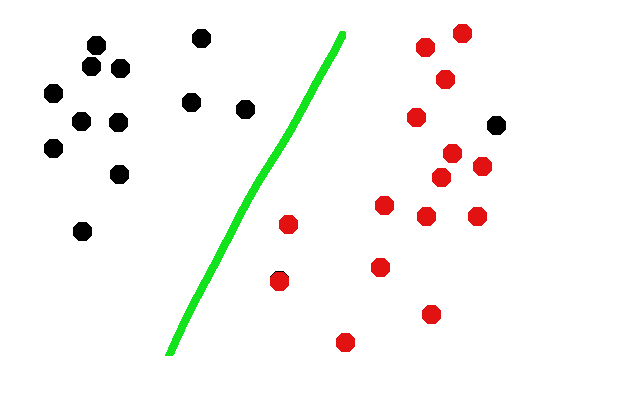
\includegraphics[scale=0.3]{images/voronoi.png}
           \end{figure}
           \end{center} 

La frontière que l'on recherche est une fonction linéaire, donc de la forme (avec un paramètre $\omega$) :\\

          \begin{center}
          $f : X -> \omega^{T}X$
          \end{center}

telle que :\\
 
         \begin{center}
         $\forall i, y_i = -1 \Rightarrow f(x_i) \leq -1$\\
         $\forall i, y_i = 1 \Rightarrow f(x_i) \geq 1$\\
         $\Leftrightarrow \forall i, y_i \times f(x_i) \geq 1$ (1)
         \end{center}

\newpage

Pour obtenir un résultat robuste, on souhaite que les deux droites $f(X) = 1$ et $f(X) = -1$ soient les plus distantes possibles. En effet, si ces deux droites sont trop proches, cela signifie que la probabilité d'erreur quant à la prédiction de la classe d'un point proche de ces droites sera importante.\\

La distance $\gamma$ entre ces deux droites se calcule de la façon suivante : soient $u, v$ deux points tels que $f(v) = 1$ et $f(u) = -1$. Alors :

      \begin{center}
      $\|f(v) - f(u)\| = \|\omega \times (v-u)\| = \|\omega\| \times \|(v-u)\| = \|\omega\| \times \|\gamma\| = \|1 - (-1)\| = 2$
      \end{center}

Finalement, le problème d'optimisation à résoudre pourrait être :\\
 
           \begin{centre}
           $max_{w}$ $\gamma = \frac{2}{\|w\|}$ avec (1) $\Leftrightarrow min_{w}$ $\|w\|$ avec (1)\\
           $\Leftrightarrow min_{w}$ $\frac{1}{2} \times \|w\|^2$ avec (1) pour faciliter les calculs
           \end{centre}

\bigskip

Un autre problème se pose si on s'arrête ici : par exemple, dans l'exemple de la frontière de Voronoi que l'on a vu ci-dessus, il n'existe pas de droite telle qu'il n'y ait que de points noirs d'un côté et que des points rouges de l'autre côté, ce qui contredit la condition (1). Pourtant, la droite dessinée en vert peut sembler acceptable comme frontière pour cet ensemble de points.\\

On tient compte de cette erreur en introduisant les variables $(z_i)_{i \leq m}$. Pour que la condition (1) soit toujours vérifiée, il faut que quand $y_i \times f(x_i) \geq 1$, $z_i = 0$ et lorsque $y_i \times f(x_i) < 1$, $z_i = 1 - y_i \times f(x_i)$. Le but étant de minimiser le nombre de ces erreurs, on utilise un paramètre $C$ constant qui permet d'insister plus ou mins sur la minimisation de ces erreurs :\\ 


           \begin{centre}
           (P) $min_{w}$ $\frac{1}{2} \times \|w\| + C \times \sum_{i \leq m}z_i$\\
           avec $\forall i, z_i \geq 0$\\
           $\forall i, y_i \times (\omega^{T} x_i) \geq 1 - z_i$\\
           \end{centre}

\bigskip

Les fonctions que l'on a introduites sont toutes convexes. Si la dimension des points $x_i$ est petite, nous allons pouvoir utiliser la méthode de Newton pour résoudre ce problème.

\section{Calcul du dual}

Calculons le lagrangien du problème (P). Soit $\lambda$ le multiplicateur de Lagrange :

              \begin{center}
              $\forall w, \lambda \in \mathbb{R}^{2m}, L(\omega, \lambda, z) = $\\
              $= \frac{1}{2} \|w\|^2 + C \times \sum_{i \leq m} z_i - \sum_{i < m} \lambda_{m+i} \times z_i$\\
              $+ \sum_{i < m} \lambda_i \times (1 - z_i - y_i \omega^{T} x_i)$\\
              \end{center}

Minimisons L par rapport à $\omega$ :\\

              \begin{center}
              $\nabla_{\omega} L(\omega, \lambda, z) = \omega + 0 + \sum_{i < m} \lambda_i \times (0$\\
              $- 0 - y_i \times x_i) = 0$\\
              $\Leftrightarrow \omega - \sum_{i < m} \lambda_i \times y_i \times x_i = 0$\\
              $\Leftrightarrow \omega = \sum_{i < m} \lambda_i \times y_i \times x_i$ (1)\\
              \end{center}

Minimisons L par rapport à $z$ :\\

              \begin{center}
              $\nabla_{z} L(\omega, \lambda, z) = 0 + C \times m - \sum_{i < m} \lambda_{m+i} $\\
              $+ \sum_{i < m} \lambda_i \times (0 - 1 - 0) = 0$\\
              $\Leftrightarrow C \times m - \sum_{i < m} \lambda_{m+i} - \sum_{i < m} \lambda_i = 0$\\
              $\Leftrightarrow  C \times m = \sum_{i < 2m} \lambda_i$ (2)\\
              \end{center}

On note alors, en injectant les valeurs de $\omega$ et de $z$ ($z \leq 0$ et $C, \lambda_i \geq 0 \forall i$, donc on prend $z=0$) dans le lagrangien :\\

              \begin{center}
              $g(\lambda) = \sum_i \lambda_i -\frac{1}{2} \times \sum_{ij} \lambda_i y_i \lambda_j y_j x_i^{T} x_j$
              \end{center}

Le problème dual est donc :\\

             \begin{center}
             $min_{\lambda \in \mathbb{R}^{m}} g(\lambda)$\\ 
             avec $\forall i, 0 \leq \lambda_i \leq C$ (vient de (2))\\
             \end{center}

On obtient la solution du primal à partir de celle du dual :

             \begin{center}
             (1) $\omega^{*} = \sum_i \lambda^{*}_i y_i x_i$
             \end{center}

\section{Utilisation de l'astuce du noyau}

Pour pouvoir trouver efficacement la solution au problème, il faut s'affranchir de la contrainte quadratique sur $\omega$.\\



\end{document}
